\documentclass[aspectratio=169, 11pt]{beamer}

% --- Packages & Setup (from the new template) ---
\usepackage[utf8]{inputenc}
\usepackage[T1]{fontenc}
\usepackage{helvet}
\renewcommand{\familydefault}{\sfdefault}
\usepackage{xcolor}
\usepackage{booktabs}
\usepackage{array}
\usepackage{graphicx}
\usepackage{tikz}
\usetikzlibrary{calc,arrows.meta,positioning}

% Left-aligned paragraph column (avoids stretched word spacing in narrow table cells)
\newcolumntype{L}[1]{>{\raggedright\arraybackslash}p{#1}}

% Images and logo live in ppt/ (one level up)
\graphicspath{{../}{./}}

% --- Branding Colors ---
\definecolor{amritaMaroon}{HTML}{A4123F}
\definecolor{maroonSoft}{HTML}{F6E3E9}
\definecolor{inkGray}{HTML}{3A3A3A}

% --- Theme Setup ---
\usetheme{Madrid}
\usecolortheme[named=amritaMaroon]{structure}
\setbeamertemplate{navigation symbols}{}
\setbeamertemplate{footline}[frame number]
\setbeamertemplate{bibliography item}[text]

% --- Reusable TikZ styles ---
\tikzset{
  flow/.style={rectangle, draw=amritaMaroon, thick, fill=maroonSoft, rounded corners=2pt,
               minimum height=0.8cm, text width=1.75cm, font=\scriptsize, align=center},
  flowdark/.style={flow, fill=amritaMaroon, text=white, font=\scriptsize\bfseries},
  arr/.style={-{Latex[length=1.8mm]}, thick, draw=amritaMaroon},
  lbl/.style={circle, draw=amritaMaroon, thick, fill=maroonSoft, minimum size=1.15cm, font=\tiny, align=center},
  lblcenter/.style={circle, draw=amritaMaroon, very thick, fill=amritaMaroon, text=white, minimum size=1.25cm, font=\tiny\bfseries, align=center},
  edg/.style={-, thick, draw=inkGray}
}

\begin{document}

% =========================================================================
% TITLE SLIDE
% =========================================================================
\begin{frame}
    \begin{tikzpicture}[remember picture,overlay]
        \node[fill=amritaMaroon, text=white, font=\bfseries\footnotesize, anchor=north east, rounded corners=2pt, inner sep=5pt]
        at ($(current page.north east) + (-0.2cm,-0.2cm)$)
        {Type 2: Application Project};
    \end{tikzpicture}

    \centering
    
\includegraphics[width=2.4cm]{logo.png}
    \vspace{0.05cm}

    {\normalsize \textbf{\textcolor{amritaMaroon}{Evaluating Graph Representations using Weisfeiler--Lehman Graph Kernels\\for Plant-Stress Classification}}} \\
    \vspace{0.05cm}
    {\footnotesize \textbf{23CSE498 -- Project Phase II (External Review)} \quad | \quad \textbf{Team Number: 49}} \\
    \vspace{0.1cm}

    \begin{table}
        \centering
        \scriptsize
        \renewcommand{\arraystretch}{1.0}
        \begin{tabular}{|c|c|l|}
            \hline
            \textbf{S.No} & \textbf{Register Number} & \textbf{Student Name} \\
            \hline
            1 & CB.SC.U4CSE23154 & Yerneni Vishnu Vardhan \\
            \hline
            2 & CB.SC.U4CSE23609 & Bala Bharath Chandra Sai \\
            \hline
            3 & CB.SC.U4CSE23610 & Chilukuri Subrahmanya Sri Prakash \\
            \hline
            4 & CB.SC.U4CSE23613 & Muppagowni Vamsidhar \\
            \hline
            5 & CB.SC.U4CSE23664 & Merugumala Sandeep \\
            \hline
        \end{tabular}
    \end{table}
    \vspace{0.05cm}

    {\footnotesize Guide: \textbf{Mr. Sriram S.}, Assistant Professor (OC), Department of CSE} \\
    \vspace{0.05cm}
    {\scriptsize \today}
\end{frame}

% =========================================================================
% GUIDE APPROVAL (Mandatory)
% =========================================================================
\begin{frame}{Guide Review \& Submission Approval}
    \framesubtitle{Confirmation of Project Review and Approval from Guide}
    \centering
    \fbox{\begin{minipage}[c][5.4cm]{0.94\textwidth}
        \centering
        \textbf{[Insert Screenshot of Guide Approval Email Here]} \\[0.3cm]
        {\footnotesize [Mandatory: Attach a clear, readable screenshot of the email received from your project guide approving this presentation and final review submission]}
    \end{minipage}}
\end{frame}

% =========================================================================
% SECTION 1: PROBLEM DEFINITION, REQUIREMENT ANALYSIS & SOLUTION DESIGN
% =========================================================================
\section{Requirements \& Solution Design}

% --- PROBLEM DEFINITION & REQUIREMENT ANALYSIS ---
\begin{frame}{1. Problem Definition \& Requirement Analysis}
    \framesubtitle{Target Problem, User Needs \& Functional / Non-Functional Requirements}
    \begin{block}{Problem Statement \& Target Stakeholders}
        \scriptsize
        \begin{itemize}
            \item \textbf{Real-World Problem:} Nutrient deficiencies (N, K, Mg and combinations), pests and diseases give visually similar leaf symptoms; misdiagnosis wastes fertiliser and yield. Standard classifiers treat leaf traits as independent numbers.
            \item \textbf{Research Question:} Which \textbf{graph representation} of leaf traits makes the \textbf{Weisfeiler--Lehman (WL) kernel} most effective for plant-stress classification, and for which diagnostic tasks?
            \item \textbf{Target Users \& Use Context:} Plant-phenotyping researchers, agronomists and extension workers; 8 crops of the OLID-I benchmark \cite{orka2023olid}.
        \end{itemize}
    \end{block}

    \begin{columns}[T]
        \column{0.53\textwidth}
        \begin{block}{Functional Requirements}
            \scriptsize
            \begin{itemize}
                \item \textbf{FR-1:} Segment the leaf and extract 38 interpretable traits per image.
                \item \textbf{FR-2:} Build 5 graph representations and WL kernels ($h=0..3$); classify stress with an SVM.
                \item \textbf{FR-3:} Hierarchical diagnosis (crop $\rightarrow$ crop-specific stress) presented in the \textbf{PlantCare AI} web portal.
            \end{itemize}
        \end{block}
        \column{0.45\textwidth}
        \begin{block}{Non-Functional Requirements}
            \scriptsize
            \begin{itemize}
                \item \textbf{NFR-1:} Leakage-free, reproducible evaluation (training-fold fitting, seed 42).
                \item \textbf{NFR-2:} CPU-only and lightweight (38 numbers per leaf); interpretable outputs; browser-based portal.
            \end{itemize}
        \end{block}
    \end{columns}
\end{frame}

% --- MOTIVATION & WL KERNEL IDEA ---
\begin{frame}{Motivation: Why Graphs and the WL Kernel?}
    \framesubtitle{Plant stress is a pattern of related traits, not a list of independent numbers}
    \begin{columns}[c]
        \column{0.56\textwidth}
        \footnotesize
        \begin{itemize}
            \item \textbf{Stress shows up as trait combinations:} e.g.\ yellowing \emph{at the leaf edge} with normal shape vs.\ \emph{uniform} pale colour.
            \item \textbf{A leaf as a graph:} each of the 38 traits is a node; edges connect related traits.
            \item \textbf{WL kernel} \cite{shervashidze2011weisfeiler}, rooted in the 1-WL isomorphism test \cite{weisfeiler1968reduction}: repeatedly relabels each node from its neighbours and compares graphs by shared neighbourhood patterns. Each pattern is a \textbf{readable trait combination}.
            \item Proven on naturally graph-structured data: malware \cite{narayanan2016contextual}, program similarity \cite{li2016detecting}, proteins \cite{borgwardt2005protein}.
            \item \textbf{Research gap:} a leaf is \emph{not} naturally a graph; how to \textbf{construct} the graph for WL on plant traits has not been studied systematically.
        \end{itemize}

        \column{0.40\textwidth}
        \centering
        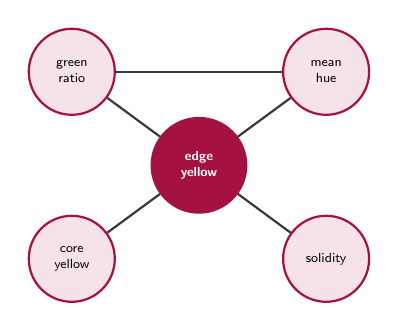
\begin{tikzpicture}[scale=0.95, every node/.style={transform shape}]
            \node[lblcenter] (y) at (0,0) {edge\\yellow};
            \node[lbl] (g) at (-1.7,1.25) {green\\ratio};
            \node[lbl] (h) at (1.7,1.25) {mean\\hue};
            \node[lbl] (c) at (-1.7,-1.25) {core\\yellow};
            \node[lbl] (s) at (1.7,-1.25) {solidity};
            \draw[edg] (y) -- (g); \draw[edg] (y) -- (h);
            \draw[edg] (y) -- (c); \draw[edg] (y) -- (s);
            \draw[edg] (g) -- (h);
        \end{tikzpicture}

        \vspace{0.1cm}
        {\scriptsize\itshape A node's label absorbs its neighbours' labels: ``edge-yellow High next to green-ratio Low''.}
    \end{columns}
\end{frame}

% --- WL FORMULATION ---
\begin{frame}{The WL Subtree Algorithm}
    \framesubtitle{Formal update rule and visual intuition \cite{weisfeiler1968reduction, shervashidze2011weisfeiler}}
    \begin{columns}[c]
        \column{0.46\textwidth}
        \begin{center}
            $\displaystyle l_i(v) = f\Big(l_{i-1}(v),\ \{\!\{\, l_{i-1}(u) : u \in N(v) \,\}\!\}\Big)$
        \end{center}
        \vspace{0.1cm}
        \scriptsize
        \begin{itemize}
            \item $l_i(v)$: label of node $v$ after iteration $i$.
            \item $N(v)$: neighbours of $v$; $\{\!\{\cdot\}\!\}$: \textbf{multiset} of their labels.
            \item $f$: compresses (own label, sorted neighbour labels) into a new compact label; the map is learned on \textbf{training graphs only}.
            \item Iterating to height $h$ captures subtrees of depth $h$ around every trait node.
        \end{itemize}

        \column{0.52\textwidth}
        \centering
        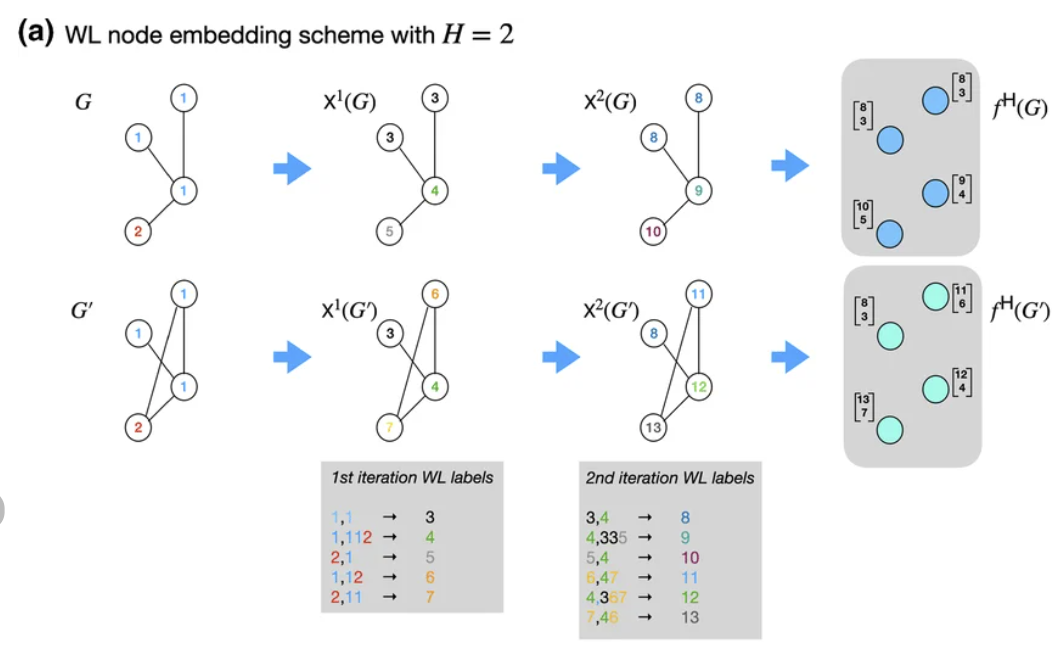
\includegraphics[width=\linewidth, height=0.68\textheight, keepaspectratio]{wl_demo.png}\\
        {\tiny\itshape Subtree neighbourhood aggregation in WL \cite{shervashidze2011weisfeiler}.}
    \end{columns}
\end{frame}

% --- END-TO-END ARCHITECTURE ---
\begin{frame}{2. End-to-End Application Architecture}
    \framesubtitle{System Architecture \& User-to-Backend Workflow Diagram}
    \centering
    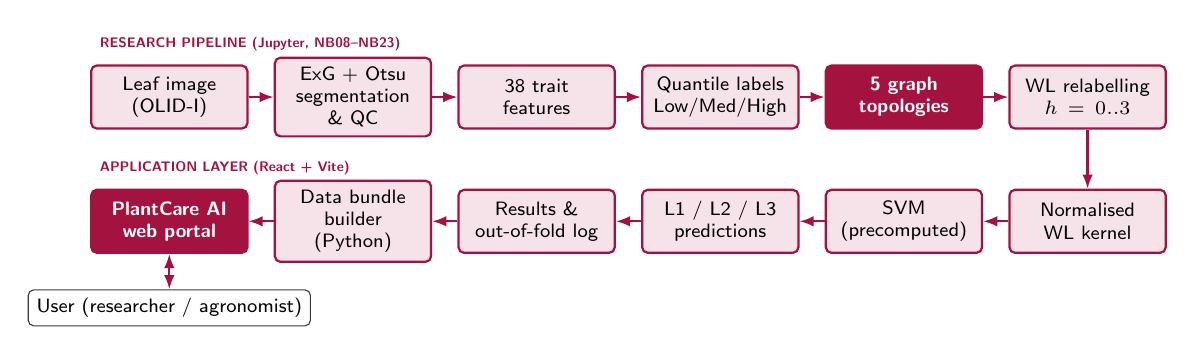
\begin{tikzpicture}[node distance=0.32cm]
        % Research pipeline (row 1)
        \node[flow] (a1) {Leaf image\\(OLID-I)};
        \node[flow, right=of a1] (a2) {ExG + Otsu\\segmentation \& QC};
        \node[flow, right=of a2] (a3) {38 trait\\features};
        \node[flow, right=of a3] (a4) {Quantile labels\\Low/Med/High};
        \node[flowdark, right=of a4] (a5) {5 graph\\topologies};
        \node[flow, right=of a5] (a6) {WL relabelling\\$h = 0..3$};
        % Row 2 (right to left)
        \node[flow, below=0.75cm of a6] (b1) {Normalised\\WL kernel};
        \node[flow, left=of b1] (b2) {SVM\\(precomputed)};
        \node[flow, left=of b2] (b3) {L1 / L2 / L3\\predictions};
        \node[flow, left=of b3] (b4) {Results \&\\out-of-fold log};
        \node[flow, left=of b4] (b5) {Data bundle\\builder (Python)};
        \node[flowdark, left=of b5] (b6) {PlantCare AI\\web portal};
        \draw[arr] (a1) -- (a2); \draw[arr] (a2) -- (a3); \draw[arr] (a3) -- (a4);
        \draw[arr] (a4) -- (a5); \draw[arr] (a5) -- (a6); \draw[arr] (a6) -- (b1);
        \draw[arr] (b1) -- (b2); \draw[arr] (b2) -- (b3); \draw[arr] (b3) -- (b4);
        \draw[arr] (b4) -- (b5); \draw[arr] (b5) -- (b6);
        % lane labels
        \node[font=\tiny\bfseries, text=amritaMaroon, anchor=south west] at ($(a1.north west)+(0,0.05)$) {RESEARCH PIPELINE (Jupyter, NB08--NB23)};
        \node[font=\tiny\bfseries, text=amritaMaroon, anchor=south west] at ($(b6.north west)+(0,0.05)$) {APPLICATION LAYER (React + Vite)};
        % user
        \node[font=\scriptsize, below=0.45cm of b6, draw=inkGray, rounded corners=2pt, inner sep=3pt] (u) {User (researcher / agronomist)};
        \draw[arr, {Latex[length=1.8mm]}-{Latex[length=1.8mm]}] (b6) -- (u);
    \end{tikzpicture}
    \vspace{0.1cm}

    \begin{block}{Architecture Summary}
        \scriptsize Each leaf flows through segmentation, trait extraction, discretisation and one of five graph constructions; WL kernels feed an SVM evaluated by cross-validation. The resulting predictions are packaged into a static data bundle that the PlantCare AI portal visualises for the user.
    \end{block}
\end{frame}

% --- ARCHITECTURAL COMPONENTS ---
\begin{frame}{3. Architectural Components \& Interface Design}
    \framesubtitle{Component Breakdown, Data Flow \& Technology Specifications}
    \begin{columns}[T]
        \column{0.50\textwidth}
        \begin{block}{Core Application Components}
            \scriptsize
            \begin{itemize}
                \item \textbf{Feature module (NB08--10):} segmentation, 38 traits, quality audit.
                \item \textbf{Graph \& WL engine (NB11--13):} 5 fold-safe topologies, WL relabelling, kernel matrices.
                \item \textbf{Classification \& evaluation (NB14--23):} kernel SVM, flat baselines, task decomposition L1--L3.
            \end{itemize}
        \end{block}

        \begin{block}{User Interaction \& Workflow Design}
            \scriptsize
            \begin{itemize}
                \item \textbf{Primary User Journey:} Dashboard $\rightarrow$ Analyze Plant (pick a leaf, step through the pipeline) $\rightarrow$ prediction $\rightarrow$ History \& Logs.
                \item \textbf{Interface Design:} Dashboard, Analyze Plant, Diagnostics, Stress Library, Crops, History \& Logs, ML Pipeline, Protocol views.
            \end{itemize}
        \end{block}

        \column{0.46\textwidth}
        \begin{block}{Data \& External Interfaces}
            \scriptsize
            \begin{itemize}
                \item \textbf{Data Storage:} feature table (4,749 leaves $\times$ 38 traits), fixed fold assignments, per-fold result CSVs.
                \item \textbf{App bundle:} summary data + out-of-fold log for all 4,387 accepted leaves.
                \item \textbf{External:} OLID-I image archive \cite{orka2023olid}.
            \end{itemize}
        \end{block}

        \begin{block}{Platform \& Deployment}
            \scriptsize
            \begin{itemize}
                \item \textbf{Stack:} Python, scikit-learn \cite{pedregosa2011scikit}, NetworkX, SciPy; React 18, Vite, Tailwind.
                \item \textbf{Target:} Jupyter on CPU (research); static web app on Vercel (portal).
            \end{itemize}
        \end{block}
    \end{columns}
\end{frame}

% =========================================================================
% SECTION 2: IMPLEMENTATION DETAILS
% =========================================================================
\section{Implementation Details}

% --- IMPLEMENTATION OVERVIEW ---
\begin{frame}{4. Implementation Details -- Overview}
    \framesubtitle{End-to-End Application Module \& Integration Status}
    \begin{table}
        \centering
        \scriptsize
        \renewcommand{\arraystretch}{1.05}
        \begin{tabular}{L{4.2cm} L{7.6cm} c}
            \toprule
            \textbf{Module} & \textbf{Implemented Features \& Scope} & \textbf{Status} \\
            \midrule
            Segmentation \& QC (NB08--10) & ExG + Otsu, morphology, ACCEPT / FAILED / SUSPICIOUS audit & Complete \\
            Feature extraction (NB08--09) & 38 traits; NaN / Inf / constant / outlier checks & Complete \\
            Graph construction (NB11) & Correlation, kNN, Feature-Family, Spatial, Hybrid (training-fold fitted) & Complete \\
            WL engine \& kernels (NB12--13) & Subtree relabelling $h=0..3$, OOV handling, normalised kernels & Complete \\
            Classification \& baselines (NB14--18) & Kernel SVM vs RF, Linear/RBF SVM, kNN on identical folds & Complete \\
            Task decomposition (NB19--23) & L1 binary, L2 per-crop, L3 crop routing + stress (nested inner CV) & Complete \\
            PlantCare AI portal & 8 views; displays recorded out-of-fold predictions & Functional \\
            \bottomrule
        \end{tabular}
    \end{table}

    \begin{block}{Prototype Environment \& Repository}
        \scriptsize
        \begin{itemize}
            \item \textbf{Execution Platform:} Python / Jupyter on a CPU workstation; portal runs in any browser (Vercel).
            \item \textbf{Source Repository:} \url{https://github.com/BharathBala21/WL_Graph_Representation}
        \end{itemize}
    \end{block}
\end{frame}

% --- DATASET & SEGMENTATION ---
\begin{frame}{Dataset, Segmentation \& Quality Control}
    \framesubtitle{OLID-I leaves \cite{orka2023olid} isolated with Excess-Green + Otsu \cite{woebbecke1995color, otsu1979threshold}}
    \begin{columns}[c]
        \column{0.50\textwidth}
        \scriptsize
        \textbf{Dataset:} 4,749 images $\cdot$ 8 crops $\cdot$ 20 conditions $\cdot$ 57 crop--condition classes.

        \vspace{0.12cm}
        \textbf{Segmentation:} $\mathrm{ExG} = 2g - r - b$ on normalised RGB, Otsu threshold, morphological cleanup, largest contour kept.

        \vspace{0.12cm}
        \textbf{Quality rule} (mask area ratio = leaf area / image area):
        \begin{center}
        \begin{tabular}{@{}ll@{}}
            \toprule
            \textbf{Condition} & \textbf{Status} \\
            \midrule
            ratio $< 0.01$ & FAILED (349) \\
            ratio $> 0.98$ & SUSPICIOUS (13) \\
            $0.01 \le$ ratio $\le 0.98$ & \textbf{ACCEPT (4,387)} \\
            \bottomrule
        \end{tabular}
        \end{center}
        \vspace{0.05cm}
        \textbf{Acceptance 92.38\%}; tomato lowest (72.68\%), ash gourd highest (99.90\%) -- a selection effect we report explicitly.

        \column{0.48\textwidth}
        \centering
        \begin{tikzpicture}
            \node[inner sep=0] (raw) {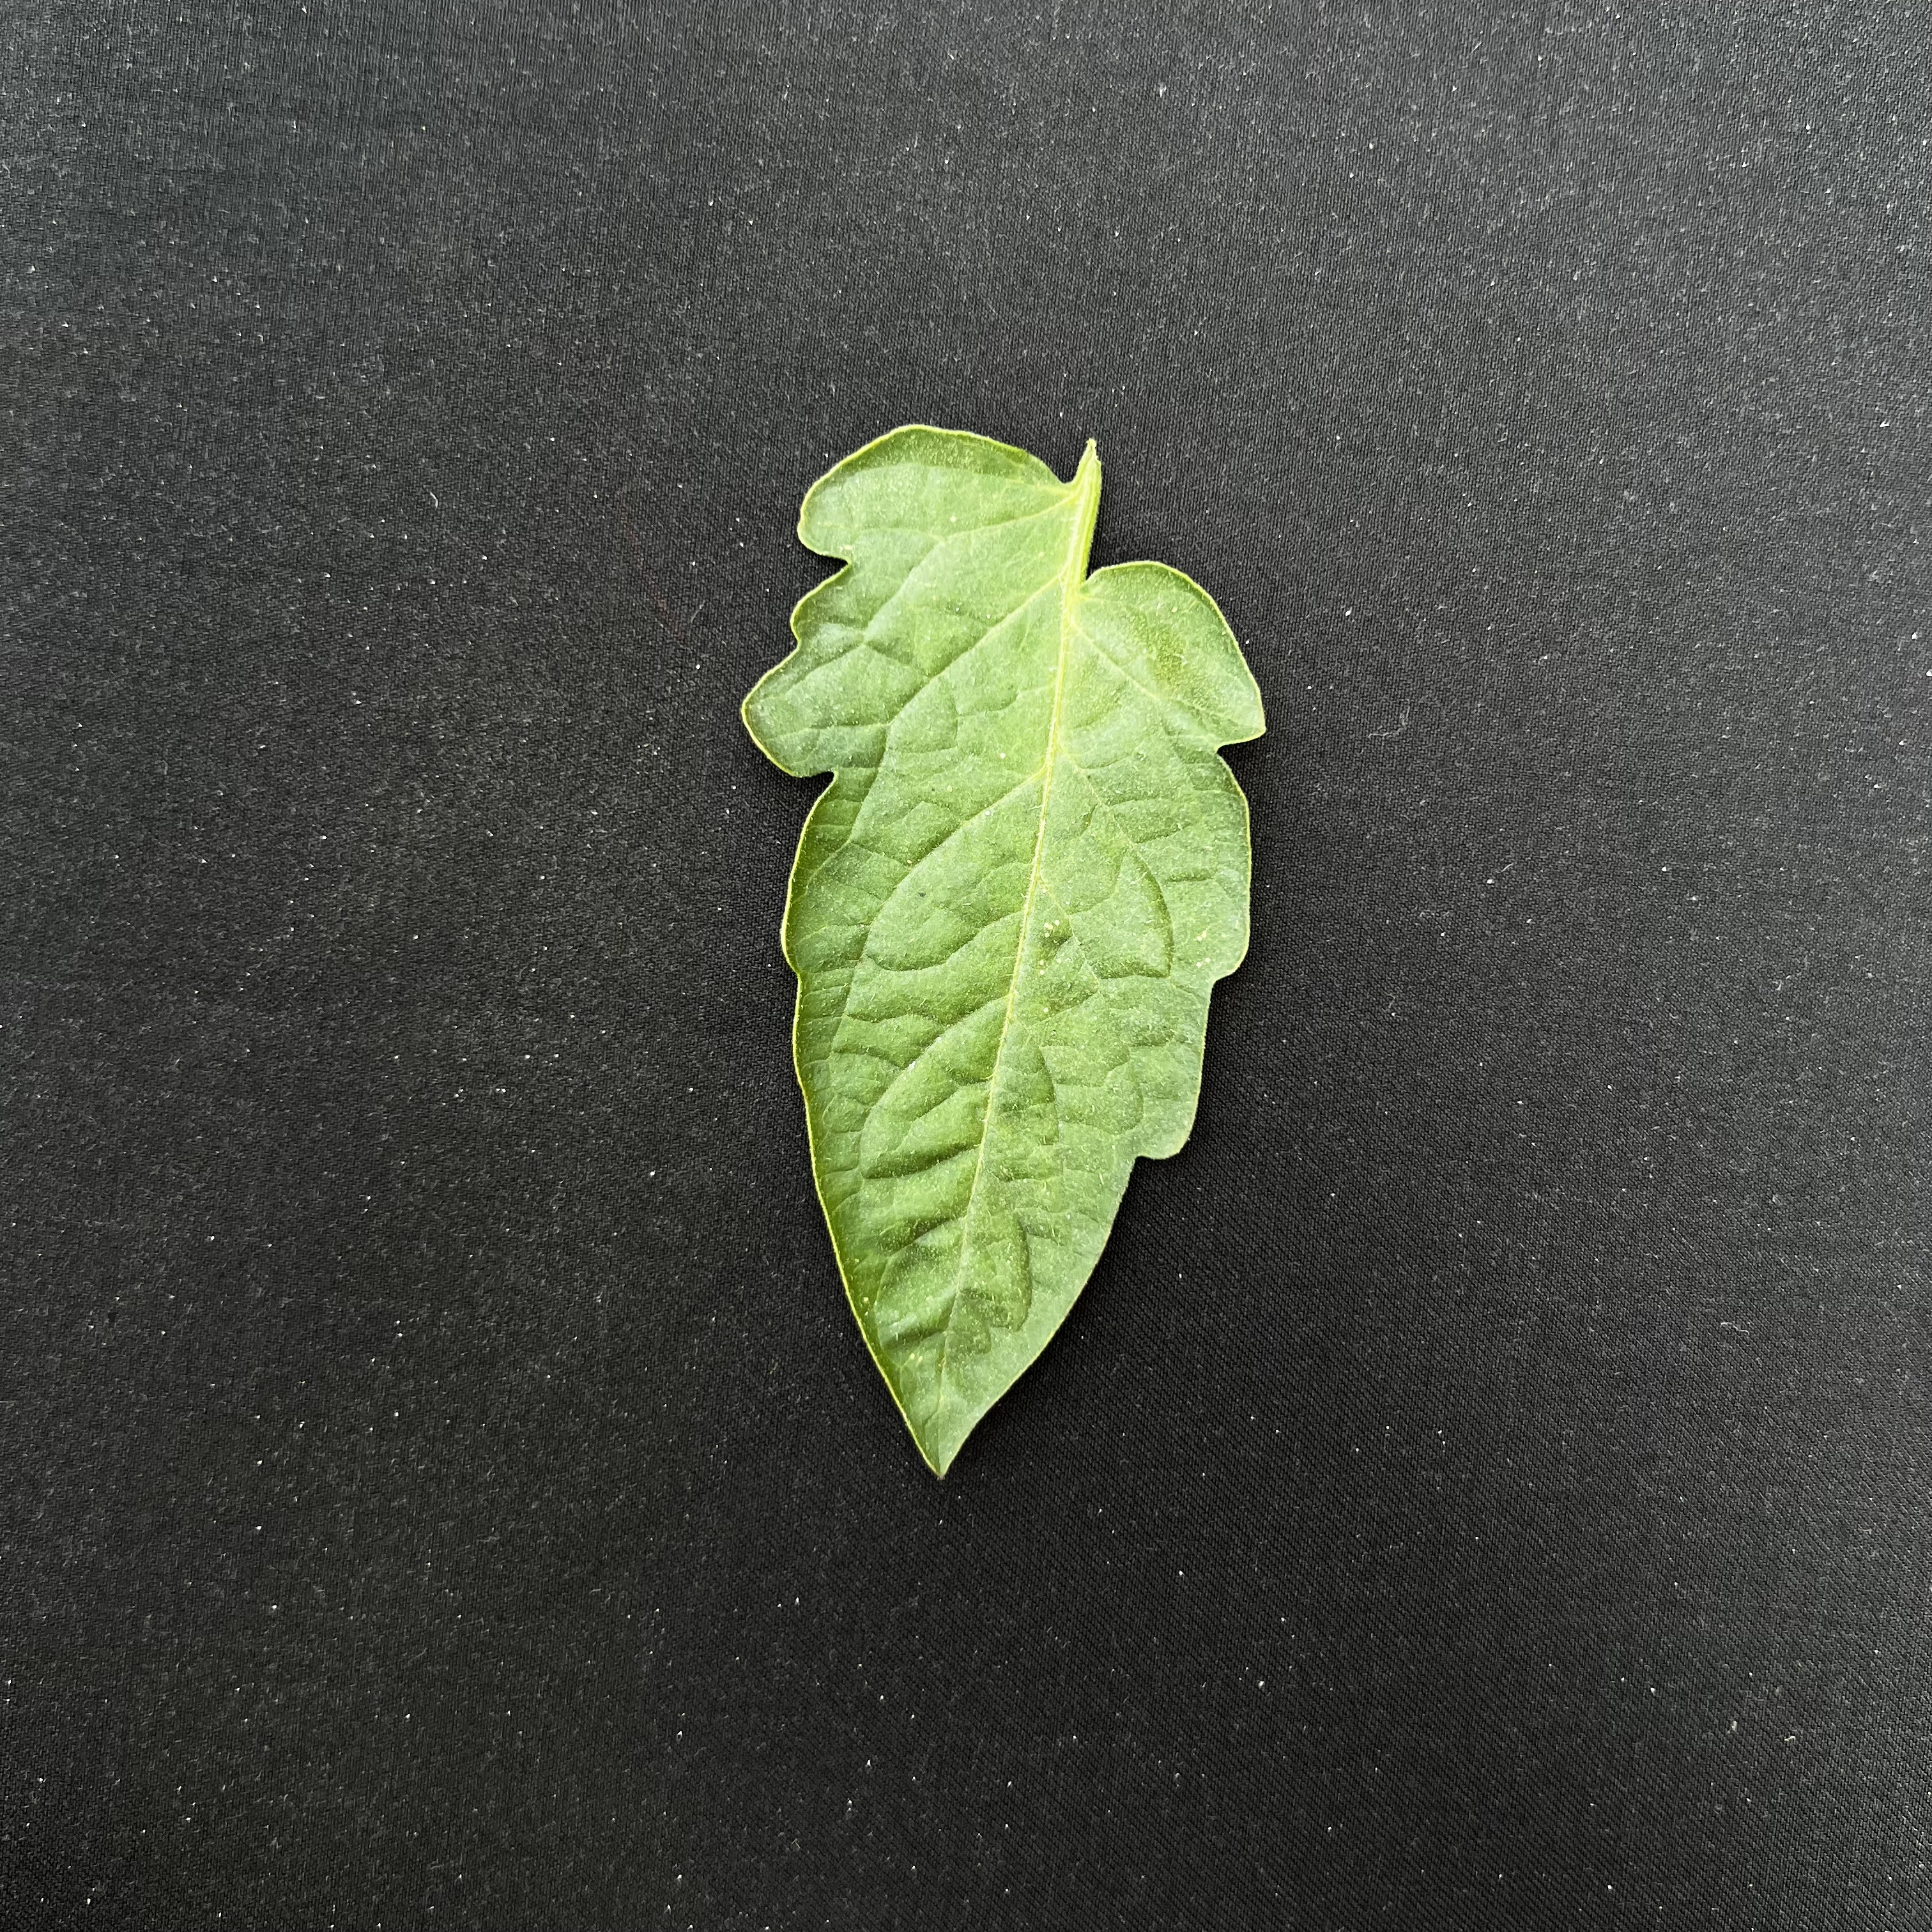
\includegraphics[height=2.8cm]{leaf_sample.JPG}};
            \node[inner sep=0, right=0.9cm of raw] (mask) {
\includegraphics[height=2.8cm]{segmentation_example.png}};
            \draw[arr] (raw) -- (mask);
            \node[below=0.1cm of raw, font=\tiny] {Raw leaf image};
            \node[below=0.1cm of mask, font=\tiny] {Binary leaf mask};
        \end{tikzpicture}\\[0.2cm]
        {\tiny\itshape Excess-Green response thresholded with Otsu; largest contour kept.}
    \end{columns}
\end{frame}

% --- FEATURES & DISCRETISATION ---
\begin{frame}{Trait Extraction \& Node Labelling}
    \framesubtitle{38 interpretable traits become the 38 nodes of every leaf graph}
    \begin{columns}[T]
        \column{0.58\textwidth}
        \scriptsize
        \renewcommand{\arraystretch}{1.15}
        \begin{tabular}{@{}L{2.5cm}c L{4.6cm}@{}}
            \toprule
            \textbf{Family} & \textbf{\#} & \textbf{Traits} \\
            \midrule
            Shape \& geometry & 10 & area, perimeter, aspect ratio, circularity, extent, solidity, convex area, axis lengths, eccentricity \\
            Colour (RGB, HSV, Lab) & 18 & mean and std of each channel \\
            Derived colour & 2 & green ratio, yellow ratio \\
            Texture (GLCM) \cite{haralick1973textural} & 4 & contrast, homogeneity, energy, correlation \\
            Spatial / regional & 4 & core / edge mean hue and yellow ratio \\
            \bottomrule
        \end{tabular}

        \column{0.38\textwidth}
        \begin{block}{Node labels for WL}
            \scriptsize
            \begin{itemize}
                \item Each trait is split into 3 quantile bins \cite{dougherty1995supervised}: \textbf{Low / Medium / High}.
                \item Label keeps trait identity, e.g.\ \texttt{mean\_H::High}.
                \item Bin edges fitted on the \textbf{training fold only}; test leaves reuse them.
            \end{itemize}
        \end{block}
        \vspace{0.1cm}
        {\scriptsize\itshape Every leaf graph has the same 38 nodes; only the node labels differ between leaves.}
    \end{columns}
\end{frame}

% --- FIVE GRAPH REPRESENTATIONS ---
\begin{frame}{The Five Graph Representations Compared}
    \framesubtitle{Same 38 nodes, different edges -- edges decide which trait patterns WL can see}
    \begin{table}
        \centering
        \scriptsize
        \renewcommand{\arraystretch}{1.3}
        \begin{tabular}{L{2.6cm} L{6.4cm} L{3.0cm} c}
            \toprule
            \textbf{Topology} & \textbf{Construction rule (training fold only)} & \textbf{Captures} & \textbf{Edges} \\
            \midrule
            Correlation & Edge if $|r| \ge 0.70$ (Pearson \cite{pearson1895notes}) & statistical co-variation & 71.8 \\
            Feature-Similarity $k$NN & Each trait linked to its $k=3$ most similar traits \cite{cover1967nearest} & similarity, no threshold & 81 \\
            Feature-Family & Cliques inside 7 families + strongest bridge between each family pair & domain knowledge & 124 \\
            Spatial / Regional & Core--core, edge--edge, core--edge links + global traits with $|r| \ge 0.60$ & \emph{where} symptoms appear & 19 \\
            Hybrid & Correlation (0.80) $\cup$ Family $\cup$ Spatial (0.70) & combined structure & 147 \\
            \bottomrule
        \end{tabular}
    \end{table}
    \vspace{0.1cm}
    \centering
    {\scriptsize Mean edge counts across the five training folds. $h = 0$ ignores edges entirely and acts as the built-in \textbf{no-structure control}.}
\end{frame}

% --- TOPOLOGY VISUALS ---
\begin{frame}{Graph Topologies Learned from the Training Data}
    \centering
    \begin{tabular}{ccc}
        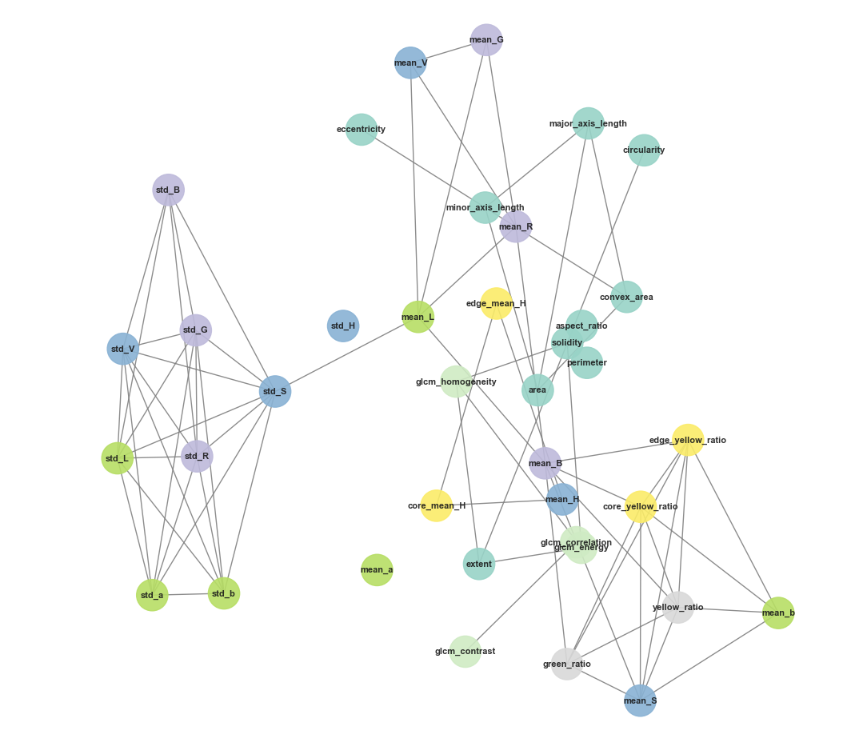
\includegraphics[height=0.33\textheight, width=0.30\textwidth, keepaspectratio]{correlation_graph.png} &
        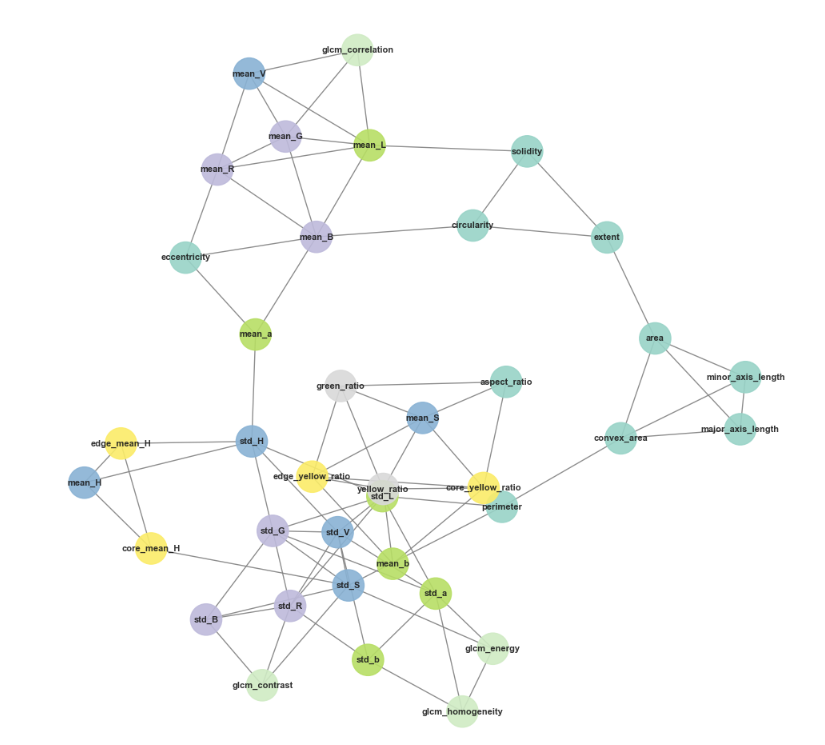
\includegraphics[height=0.33\textheight, width=0.30\textwidth, keepaspectratio]{knn_Graph.png} &
        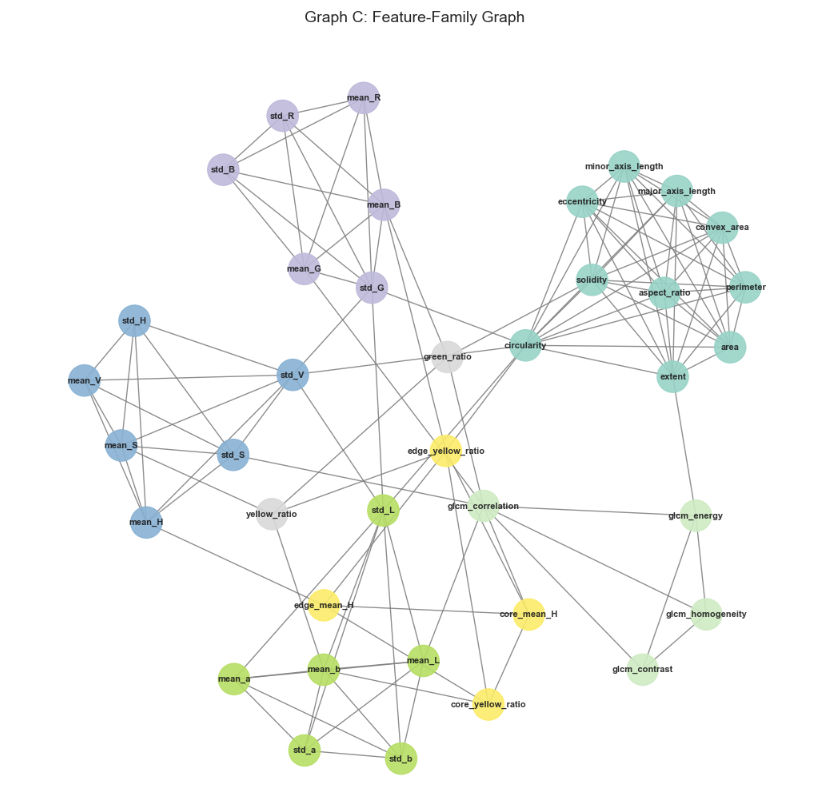
\includegraphics[height=0.33\textheight, width=0.30\textwidth, keepaspectratio]{feature_family.png} \\
        {\scriptsize Correlation} & {\scriptsize Feature-Similarity $k$NN} & {\scriptsize Feature-Family} \\[0.1cm]
        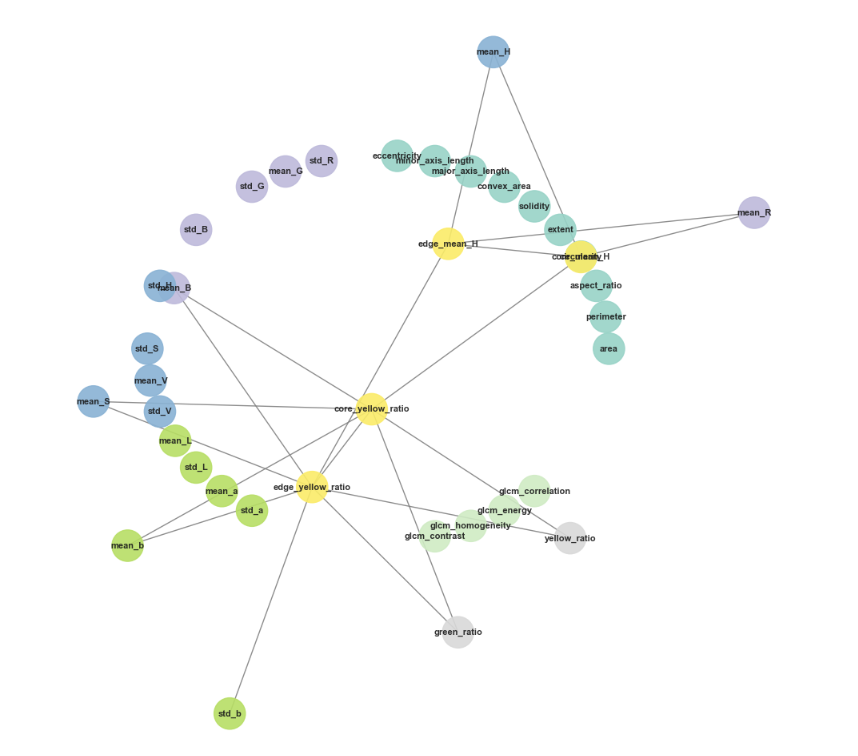
\includegraphics[height=0.33\textheight, width=0.30\textwidth, keepaspectratio]{spatial_graph.png} &
        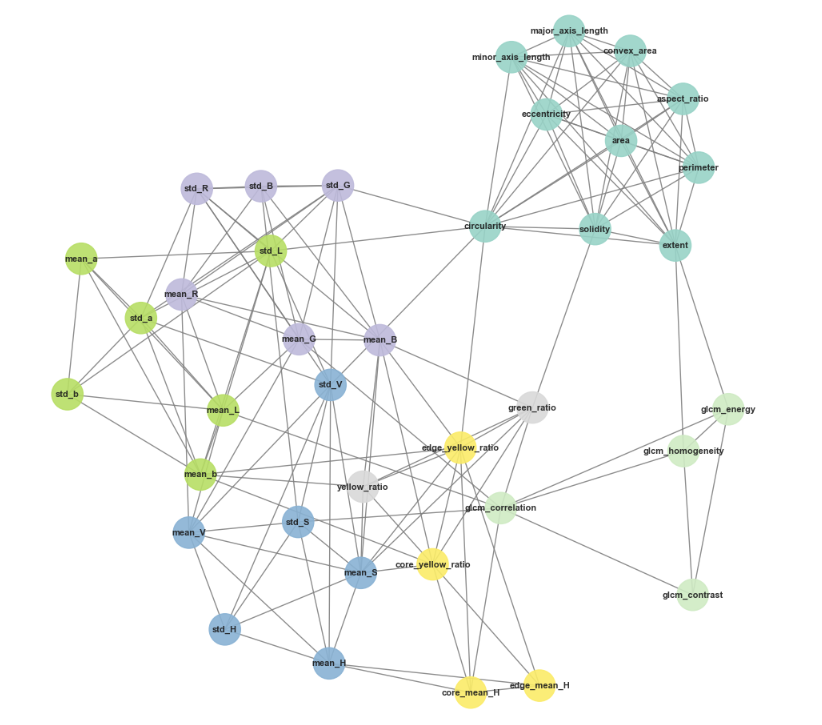
\includegraphics[height=0.33\textheight, width=0.30\textwidth, keepaspectratio]{hybrid_graph.png} &
        \begin{minipage}[b][0.30\textheight][c]{0.28\textwidth}
            \scriptsize\itshape Sparse (Spatial, 19 edges) to dense (Hybrid, 147 edges): density changes the size and specificity of the WL pattern vocabulary.
        \end{minipage} \\
        {\scriptsize Spatial / Regional} & {\scriptsize Hybrid} & \\
    \end{tabular}
\end{frame}

% --- WL VECTOR -> KERNEL -> SVM ---
\begin{frame}{From WL Patterns to Classification}
    \framesubtitle{Subtree vector $\rightarrow$ normalised kernel $\rightarrow$ SVM \cite{shervashidze2011weisfeiler, scholkopf2002learning, cortes1995support}}
    \begin{columns}[T]
        \column{0.50\textwidth}
        \scriptsize
        \textbf{1. WL subtree vector} (counts of every label, iterations $0..h$):
        \[ \phi(G) = \big[\mathbf{c}_0(G) \,\|\, \mathbf{c}_1(G) \,\|\, \cdots \,\|\, \mathbf{c}_h(G)\big] \]
        \textbf{2. Kernel matrices:}
        \[ K_{\text{train}} = \Phi_{\text{train}}\Phi_{\text{train}}^{T}, \qquad K_{\text{test}} = \Phi_{\text{test}}\Phi_{\text{train}}^{T} \]
        \textbf{3. Cosine normalisation:}
        \[ K_{\text{norm}}(i,j) = \frac{K(i,j)}{\sqrt{K(i,i)\,K(j,j)}} \]

        \column{0.46\textwidth}
        \begin{block}{Classifier}
            \scriptsize
            \begin{itemize}
                \item \texttt{SVC(kernel='precomputed')} \cite{chang2011libsvm}, $C=1$, \textbf{class-balanced} weights (healthy leaves are the minority).
                \item Test patterns never seen in training are \textbf{out-of-vocabulary} and contribute zero.
            \end{itemize}
        \end{block}
        \begin{block}{Evaluation grid}
            \scriptsize 5 topologies $\times$ 4 heights ($h=0..3$) $\times$ 5 folds = \textbf{100 kernel runs} per task.
        \end{block}
    \end{columns}
\end{frame}

% --- EVALUATION PROTOCOL & DECOMPOSITION ---
\begin{frame}{Evaluation Protocol \& Task Decomposition}
    \framesubtitle{Matching the representation to the diagnostic task}
    \begin{columns}[T]
        \column{0.46\textwidth}
        \begin{block}{Protocol}
            \scriptsize
            \begin{itemize}
                \item Stratified 5-fold CV \cite{kohavi1995study}, seed 42; \textbf{identical folds} for every model.
                \item Leakage-safe: bins, edges, WL vocabulary and scalers fitted on the training fold.
                \item Baselines on the same 38 traits: Random Forest \cite{breiman2001random}, Linear SVM, RBF SVM, $k$NN.
                \item Primary metric \textbf{Macro-F1}; also accuracy, balanced accuracy, ROC-AUC.
            \end{itemize}
        \end{block}

        \column{0.50\textwidth}
        \scriptsize
        \renewcommand{\arraystretch}{1.3}
        \begin{tabular}{@{}l L{5.2cm}@{}}
            \toprule
            \textbf{Level} & \textbf{Task} \\
            \midrule
            Full & 57-class crop + condition \\
            \textbf{L1} & Healthy vs stressed, all crops (4,387 leaves) \\
            \textbf{L2} & Healthy vs stressed inside each crop \\
            \textbf{L3} & Stage 1 crop routing $\rightarrow$ Stage 2 crop-specific stress model; topology chosen by \textbf{nested inner CV} \\
            \bottomrule
        \end{tabular}

        \vspace{0.15cm}
        {\scriptsize\itshape Why decompose: crop identity is easy ($\approx$92\%), condition is the bottleneck ($\approx$60\%).}
    \end{columns}
\end{frame}

% --- RESULTS: 57-CLASS ---
\begin{frame}{Results I: Full 57-Class Task}
    \framesubtitle{Topology matters -- but flat baselines win on the fine-grained task}
    \begin{columns}[c]
        \column{0.56\textwidth}
        \scriptsize
        \renewcommand{\arraystretch}{1.12}
        \begin{tabular}{@{}lcc@{}}
            \toprule
            \textbf{Model} & \textbf{Accuracy (\%)} & \textbf{Macro-F1 (\%)} \\
            \midrule
            Random Forest & 58.54 $\pm$ 1.47 & \textbf{54.99 $\pm$ 1.35} \\
            Linear SVM & 48.55 $\pm$ 2.10 & 47.20 $\pm$ 2.04 \\
            RBF SVM & 45.54 $\pm$ 1.97 & 43.07 $\pm$ 1.55 \\
            $k$NN ($k=5$) & 48.76 $\pm$ 0.85 & 41.02 $\pm$ 1.05 \\
            \midrule
            WL: Hybrid, $h=2$ & 44.31 $\pm$ 0.72 & \textbf{42.79 $\pm$ 0.95} \\
            WL: Feature-Family, $h=2$ & 43.86 $\pm$ 1.05 & 42.35 $\pm$ 1.06 \\
            WL: $k$NN, $h=2$ & 44.15 $\pm$ 1.07 & 42.33 $\pm$ 1.15 \\
            WL: Correlation, $h=2$ & 41.08 $\pm$ 2.09 & 39.84 $\pm$ 2.89 \\
            WL: Spatial, $h=3$ & 40.30 $\pm$ 0.93 & 39.30 $\pm$ 1.01 \\
            WL: any topology, $h=0$ & 37.36 $\pm$ 0.80 & 35.01 $\pm$ 0.54 \\
            \bottomrule
        \end{tabular}

        \column{0.40\textwidth}
        \begin{block}{Observations}
            \scriptsize
            \begin{itemize}
                \item Adding structure helps: $h=0 \rightarrow h=2$ gives up to \textbf{+7.8 pts} Macro-F1.
                \item Hybrid, Family and $k$NN are within 0.5 pts; Spatial (sparsest) is weakest.
                \item Random Forest leads by $\approx$12 pts; one reason: 3-bin labels make 30\% of leaves share an identical $h=0$ pattern.
                \item $\Rightarrow$ motivates task decomposition.
            \end{itemize}
        \end{block}
    \end{columns}
    \vspace{0.05cm}
    {\tiny Mean $\pm$ SD over 5 folds; best height per topology shown.}
\end{frame}

% --- RESULTS: LEVEL 1 ---
\begin{frame}{Results II: Level 1 -- Healthy vs Stressed (4,387 leaves)}
    \framesubtitle{Graph structure becomes competitive once the task is simplified}
    \begin{columns}[c]
        \column{0.58\textwidth}
        \scriptsize
        \renewcommand{\arraystretch}{1.12}
        \begin{tabular}{@{}lcccc@{}}
            \toprule
            \textbf{Model} & \textbf{Acc} & \textbf{Macro-F1} & \textbf{Bal.\ Acc} & \textbf{AUC} \\
            \midrule
            WL: Hybrid, $h=3$ & 81.60 & \textbf{69.69} & 72.19 & 0.813 \\
            WL: Feature-Family, $h=3$ & 80.92 & 69.14 & 72.12 & 0.812 \\
            WL: Hybrid, $h=2$ & 79.71 & 68.74 & 73.03 & 0.814 \\
            WL: $k$NN, $h=3$ & 77.87 & 67.37 & 72.91 & 0.808 \\
            Flat RBF SVM & 74.49 & 66.42 & \textbf{76.07} & 0.843 \\
            Flat Random Forest & \textbf{86.78} & 65.22 & 61.82 & \textbf{0.868} \\
            WL: Correlation, $h=3$ & 70.94 & 62.16 & 70.68 & 0.778 \\
            WL: Spatial, $h=2$ & 70.64 & 62.16 & 71.13 & 0.791 \\
            WL: any topology, $h=0$ & 67.47 & 60.07 & 70.59 & 0.759 \\
            \bottomrule
        \end{tabular}

        \column{0.38\textwidth}
        \begin{block}{Observations}
            \scriptsize
            \begin{itemize}
                \item Mean Macro-F1 rises with depth: $h$ = 0 / 1 / 2 / 3 $\rightarrow$ 60.1 / 63.6 / 65.5 / 66.1.
                \item Hybrid and Family give the best Macro-F1.
                \item RF has higher accuracy and AUC but finds only 25\% of healthy leaves; RBF has the best balanced accuracy.
                \item Best WL row is chosen on the evaluation folds (exploratory).
            \end{itemize}
        \end{block}
    \end{columns}
\end{frame}

% --- RESULTS: LEVEL 2 & 3 ---
\begin{frame}{Results III: Level 2 (per crop) \& Level 3 (hierarchical)}
    \framesubtitle{The most suitable graph representation depends on the crop}
    \begin{columns}[T]
        \column{0.58\textwidth}
        \scriptsize
        \renewcommand{\arraystretch}{1.08}
        \begin{tabular}{@{}llccc@{}}
            \toprule
            \textbf{Crop} & \textbf{Best WL topology} & \textbf{WL} & \textbf{RF} & \textbf{RBF} \\
            \midrule
            Cucumber & Family, $h=2$ & \textbf{0.852} & 0.804 & 0.681 \\
            Snake gourd & Hybrid, $h=3$ & \textbf{0.778} & 0.718 & 0.692 \\
            Tomato & Correlation, $h=2$ & 0.776 & \textbf{0.794} & 0.786 \\
            Eggplant & Hybrid, $h=3$ & \textbf{0.750} & 0.695 & 0.694 \\
            Bottle gourd & Hybrid, $h=3$ & \textbf{0.719} & 0.636 & 0.711 \\
            Bitter gourd & $k$NN, $h=3$ & 0.662 & 0.644 & \textbf{0.667} \\
            Ash gourd & Family, $h=2$ & \textbf{0.646} & 0.550 & 0.644 \\
            Ridge gourd & Hybrid, $h=1$ & 0.548 & 0.458 & \textbf{0.556} \\
            \bottomrule
        \end{tabular}

        \vspace{0.05cm}
        {\tiny Macro-F1, healthy vs stressed within each crop. WL topology selected on the evaluation folds; baselines at default settings.}

        \column{0.38\textwidth}
        \begin{block}{Level 3 (nested inner CV)}
            \scriptsize
            \begin{itemize}
                \item Stage-1 crop routing: \textbf{91.84\%} accuracy.
                \item End-to-end stress Macro-F1: \textbf{0.6825 $\pm$ 0.0132}.
                \item Perfect-routing (oracle): 0.6864 $\Rightarrow$ routing costs only \textbf{0.004}.
            \end{itemize}
        \end{block}
        \begin{block}{Takeaway}
            \scriptsize Hybrid wins 4 crops, Family 2, Correlation and $k$NN 1 each: \textbf{no single topology suits every crop}.
        \end{block}
    \end{columns}
\end{frame}

% =========================================================================
% SECTION 3: FUNCTIONAL TESTING & DEMONSTRATION
% =========================================================================
\section{Functional Testing \& Demonstration}

\begin{frame}{6. Functional Testing \& Verification Results}
    \framesubtitle{End-to-End Feature Verification \& Test Case Summary}
    \begin{table}
        \centering
        \scriptsize
        \renewcommand{\arraystretch}{1.05}
        \begin{tabular}{L{3.4cm} L{4.0cm} L{5.4cm} c}
            \toprule
            \textbf{Test Case} & \textbf{Input / Action} & \textbf{Verified Outcome} & \textbf{Status} \\
            \midrule
            TC-01: Data integrity & 4,387 accepted leaves, 38 traits & 0 NaN, 0 Inf, no constant features & Pass \\
            TC-02: Leakage safety & Fit bins / edges / WL maps & Training-fold only; validation never used & Pass \\
            TC-03: Kernel validity & 100 kernel configurations & Symmetric, PSD, finite, normalised diagonal $= 1$ & Pass \\
            TC-04: Unseen patterns & Test signatures absent in training & Treated as OOV, zero contribution, no failure & Pass \\
            TC-05: Coverage \& determinism & Full 5-fold run, repeated & 105/105 fold runs; 4,387/4,387 predictions; identical reruns & Pass \\
            TC-06: Portal workflow & Select a dataset leaf & Pipeline steps and recorded out-of-fold prediction shown & Pass \\
            \bottomrule
        \end{tabular}
    \end{table}

    \begin{block}{Application Verification Summary}
        \scriptsize
        \begin{itemize}
            \item \textbf{Functional Verification:} each stage runs automated PASS/FAIL checks in its notebook before results are recorded.
            \item \textbf{Operational Notes:} CPU-only; the portal shows recorded predictions -- uploaded images are previewed, not yet classified live.
        \end{itemize}
    \end{block}
\end{frame}

\begin{frame}{7. Working Prototype Demonstration}
    \framesubtitle{PlantCare AI -- End-to-End Walkthrough \& Visual Evidence}
    \begin{columns}[T]
        \column{0.48\textwidth}
        \centering
        \fbox{\begin{minipage}[c][4.6cm]{0.94\textwidth}
            \centering
            \textbf{[Insert Screenshot 1: PlantCare AI Dashboard]} \\[0.2cm]
            {\scriptsize Dataset overview, crop cards, topology comparison}
        \end{minipage}}

        \column{0.48\textwidth}
        \centering
        \fbox{\begin{minipage}[c][4.6cm]{0.94\textwidth}
            \centering
            \textbf{[Insert Screenshot 2: Analyze Plant -- Prediction View]} \\[0.2cm]
            {\scriptsize Pipeline walkthrough and recorded out-of-fold prediction}
        \end{minipage}}
    \end{columns}
    \vspace{0.2cm}

    \begin{block}{Live Demonstration Scenario}
        \scriptsize Select a tomato leaf in \emph{Analyze Plant} $\rightarrow$ step through segmentation, traits, graph, WL and SVM $\rightarrow$ view the crop route and stress prediction $\rightarrow$ open \emph{History \& Logs} (all 4,387 leaves) and \emph{Diagnostics} (topology and WL-height comparisons).
    \end{block}
\end{frame}

% =========================================================================
% SECTION 4: TECHNICAL KNOWLEDGE
% =========================================================================
\section{Technical Knowledge}

\begin{frame}{8. Technical Justification \& Architectural Decisions}
    \framesubtitle{Platform Rationale, Engineering Trade-offs \& Operational Considerations}
    \begin{columns}[T]
        \column{0.48\textwidth}
        \begin{block}{1. Platform \& Technology Justification}
            \scriptsize
            \begin{itemize}
                \item In-house WL engine (NetworkX + SciPy sparse) so the label map is learned on training folds only and unseen patterns are handled explicitly.
                \item Precomputed-kernel SVM: any graph kernel plugs in unchanged; static React portal needs no server.
            \end{itemize}
        \end{block}

        \begin{block}{2. Design Trade-offs}
            \scriptsize
            \begin{itemize}
                \item 3-bin labels: interpretable and robust, but lose magnitude detail.
                \item Higher $h$: richer patterns but vocabulary explodes (Hybrid $h=3$ $\approx$ 259k features) with no gain.
            \end{itemize}
        \end{block}

        \column{0.48\textwidth}
        \begin{block}{3. Reliability \& Safety Measures}
            \scriptsize
            \begin{itemize}
                \item Quality flags reject failed segmentations before modelling.
                \item Class-balanced SVM protects the healthy minority; portal shows only out-of-fold (never training) predictions.
            \end{itemize}
        \end{block}

        \begin{block}{4. Operational Constraints \& Future Scope}
            \scriptsize
            \begin{itemize}
                \item Segmentation acceptance varies by crop (tomato 72.7\%).
                \item Next: nested CV with tuned baselines, richer node labels, live inference in the portal.
            \end{itemize}
        \end{block}
    \end{columns}
\end{frame}

\begin{frame}{Key Findings \& Conclusion}
    \begin{columns}[T]
        \column{0.62\textwidth}
        \footnotesize
        \begin{enumerate}
            \item \textbf{Graph structure carries signal:} every topology improves on the no-structure control ($h=0$) in the 57-class and Level-1 experiments.
            \item \textbf{Representation matters:} Hybrid and Feature-Family are strongest overall; the sparse Spatial graph is weakest.
            \item \textbf{No universal winner:} the best topology changes with the crop (Hybrid, Family, Correlation, $k$NN).
            \item \textbf{Task granularity decides competitiveness:} flat Random Forest leads on 57 classes; WL is competitive on stress detection (L1--L3).
            \item \textbf{Deliverable:} a leakage-safe, interpretable pipeline and the PlantCare AI portal.
        \end{enumerate}

        \column{0.34\textwidth}
        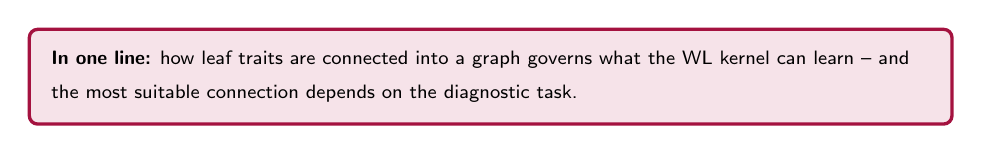
\begin{tikzpicture}
            \node[rectangle, draw=amritaMaroon, very thick, fill=maroonSoft, rounded corners=3pt,
                  inner sep=8pt, text width=0.92\columnwidth, align=flush left] {
                \scriptsize\textbf{In one line:} how leaf traits are connected into a graph governs what the WL kernel can learn -- and the most suitable connection depends on the diagnostic task.
            };
        \end{tikzpicture}
    \end{columns}
\end{frame}

% =========================================================================
% REFERENCES & THANK YOU
% =========================================================================
\section{References}
\begin{frame}[allowframebreaks]{References}
    \tiny
    \bibliographystyle{ieeetr}
    \bibliography{ref}
\end{frame}

\begin{frame}
    \centering
    {\Huge \textbf{\textcolor{amritaMaroon}{Thank You}}} \\[0.4cm]
    {\large \textbf{Questions \& Viva Voce}}
\end{frame}

\end{document}
